% =====================================================================
% Live Mandi Price Advisor -- Project Report
% Brainware University -- BTech CSE (AI/ML) Capstone Project
% Format follows: Project_Report_Template_BWU.docx (official BWU format)
%
% This is a LIVING document: update the relevant \input{} files each
% review period rather than rewriting the whole report. See README.md
% in this folder for the review-period workflow.
% =====================================================================

\documentclass[12pt,a4paper]{report}

% ---------- Page geometry (A4, standard academic margins) ----------
\usepackage[a4paper,left=1.5in,right=1in,top=1in,bottom=1in]{geometry}

% ---------- Core packages ----------
\usepackage{graphicx}
\usepackage{setspace}
\usepackage{titlesec}
\usepackage{tocloft}
\usepackage[hidelinks]{hyperref}
\usepackage{enumitem}
\usepackage{longtable}
\usepackage{array}
\usepackage{booktabs}
\usepackage{amsmath}
\usepackage{amssymb}
\usepackage{fancyhdr}
\usepackage{xcolor}
\usepackage{caption}
\usepackage{tikz}
\usetikzlibrary{arrows.meta}
\usepackage[nottoc]{tocbibind} % include References in TOC, not List of Figs/Tables again
\usepackage[numbers]{natbib}

% ---------- Chapter/section title style ----------
\titleformat{\chapter}[display]{\normalfont\bfseries\centering\Large}{\Large\thechapter.}{6pt}{\Large}
\titlespacing*{\chapter}{0pt}{0pt}{20pt}

% ---------- Header/footer ----------
\pagestyle{fancy}
\fancyhf{}
\fancyfoot[C]{\thepage}
\renewcommand{\headrulewidth}{0pt}

% ---------- Document variables (EDIT THESE per review / final report) ----------
\newcommand{\ProjectTitle}{Live Mandi Price Advisor: A Real-Time Data-Driven Forecasting and Sell/Hold Advisory System for Indian Farmers}
\newcommand{\SubmissionMonthYear}{August 2026}
\newcommand{\DegreeName}{BACHELOR OF TECHNOLOGY}
\newcommand{\BranchOfStudy}{Computer Science \& Engineering (Artificial Intelligence \& Machine Learning)}
\newcommand{\UniversityName}{BRAINWARE UNIVERSITY}
\newcommand{\UniversityAddress}{398, Ramkrishnapur Road, Barasat, North 24 Parganas, Kolkata - 700 125}
\newcommand{\SupervisorName}{Dr. Biswarup Mukherjee}
\newcommand{\SupervisorDesignation}{Professor \& Head of the Department}
\newcommand{\HODName}{Dr. Biswarup Mukherjee}
\newcommand{\HODDesignation}{Professor \& Head of the Department}
\newcommand{\DeptName}{Computer Science \& Engineering (Artificial Intelligence \& Machine Learning)}
\newcommand{\ReviewLabel}{Review 1}

\begin{document}

% ---------------------------------------------------------------
% FRONT MATTER (roman numerals, no chapter numbering)
% ---------------------------------------------------------------
\pagenumbering{roman}

% Title page -- kept as ONE continuous page (the source .docx template had
% the "BRAINWARE UNIVERSITY" header orphaned alone on a near-blank page
% due to a stray page break; that defect is intentionally not replicated here).
\begin{titlepage}
\centering
\thispagestyle{empty}

\vspace*{0.3cm}
\Large\bfseries A PROJECT REPORT\\[0.3cm]
\normalsize\normalfont ON\\[0.6cm]

{\LARGE\bfseries \ProjectTitle \par}
\vspace{0.8cm}

\normalsize\textit{Submitted by}\\[0.3cm]
{\large\bfseries
Tanmoy Maiti\\
Arnab Das\\
Raja Kumar\\
Aditya Bharati
\par}

\vspace{0.8cm}
\normalsize \textit{in partial fulfillment for the award of the degree of}\\[0.3cm]
{\large\bfseries \DegreeName \par}
\vspace{0.3cm}
\normalsize \textit{in}\\[0.2cm]
{\large\bfseries \BranchOfStudy \par}

\vfill


\includegraphics[width=2.2cm]{images/bwu_logo.jpg}\\[0.3cm]
{\large\bfseries \UniversityName \par}
\textit{\UniversityAddress}\\[0.5cm]
\ReviewLabel{} \textbar\ \SubmissionMonthYear

\end{titlepage}

\chapter*{Bonafide Certificate}
\addcontentsline{toc}{chapter}{Bonafide Certificate}
\thispagestyle{empty}
\begin{center}

\includegraphics[width=1.6cm]{images/bwu_logo.jpg}\\[0.2cm]
{\bfseries \UniversityName}\\
\textit{\UniversityAddress}\\[0.4cm]
{\bfseries [\DeptName]}\\[0.3cm]
\underline{\bfseries BONAFIDE CERTIFICATE}
\end{center}

\vspace{0.5cm}
\doublespacing
\noindent Certified that this project report \textbf{``\ProjectTitle''} is the bonafide work of \textbf{``Tanmoy Maiti, Arnab Das, Raja Kumar, Aditya Bharati''} who carried out the project work under my supervision.
\singlespacing

\vspace{2.5cm}

% Fixed: both columns now have the SAME number of rows (Signature / Name /
% Role / Academic Designation / Department / Address), symmetric left-right --
% the source template had an extra "Academic Designation" line only on the
% Supervisor side, which pushed the Department/Address rows out of alignment
% between the two columns.
\noindent
\begin{minipage}[t]{0.48\textwidth}
\underline{\hspace{4cm}}\\
\textbf{SIGNATURE}\\[0.5cm]
\HODName\\
\textbf{HEAD OF THE DEPARTMENT}\\
\HODDesignation\\
\DeptName\\
\UniversityAddress
\end{minipage}
\hfill
\begin{minipage}[t]{0.48\textwidth}
\underline{\hspace{4cm}}\\
\textbf{SIGNATURE}\\[0.5cm]
\SupervisorName\\
\textbf{SUPERVISOR}\\
\SupervisorDesignation\\
\DeptName\\
\UniversityAddress
\end{minipage}

\vspace{1cm}
\noindent\textit{Note: The Head of the Department and Project Supervisor are the same
individual for this project. Both signature blocks are retained per the
required certificate format.}

\chapter*{Abstract}
\addcontentsline{toc}{chapter}{Abstract}

% TODO: Replace with a 200-300 word abstract once implementation results
% exist (typically finalized closer to the final report, not Review 1).
Small and marginal farmers in India routinely sell their produce without
reliable knowledge of prevailing prices across nearby markets (mandis),
leading to distress selling and avoidable income loss. This project,
\textit{\ProjectTitle}, proposes a system that combines historical and
live commodity price data from the Government of India's Agmarknet
platform with time-series forecasting (Facebook Prophet) to generate
short-term price forecasts and an actionable Sell/Hold recommendation
for individual (commodity, mandi) pairs. The system is exposed through
a two-page web application -- an overview dashboard and an interactive,
state-wise prediction interface -- allowing farmers to compare prices
across nearby markets before deciding when and where to sell. This
report presents the problem motivation, a review of existing approaches,
and the proposed system architecture, data pipeline, and machine
learning design as developed to date.

\vspace{1cm}
\noindent\textbf{Keywords:} Agricultural price forecasting, Agmarknet,
Prophet time-series model, distress selling, farmer decision support,
mandi price comparison.


\clearpage
\tableofcontents

\clearpage
\listoftables

\clearpage
\listoffigures

\clearpage
\chapter*{List of Symbols, Abbreviations and Nomenclature}
\addcontentsline{toc}{chapter}{List of Symbols, Abbreviations and Nomenclature}

\begin{longtable}{@{}p{3.5cm}p{10cm}@{}}
\toprule
\textbf{Abbreviation} & \textbf{Full Form} \\
\midrule
\endhead
ML & Machine Learning \\
API & Application Programming Interface \\
CEDA & Centre for Economic Data and Analysis (Ashoka University) \\
FAQ & Fair Average Quality (Agmarknet grading term) \\
MAE & Mean Absolute Error \\
CI & Continuous Integration \\
REST & Representational State Transfer \\
UI & User Interface \\
UX & User Experience \\
CRUD & Create, Read, Update, Delete \\
\bottomrule
\end{longtable}

% TODO: expand this list as new domain-specific terms/abbreviations are
% introduced in later chapters/reviews.


% ---------------------------------------------------------------
% MAIN CHAPTERS (arabic numerals, per BWU-required chapter order)
% ---------------------------------------------------------------
\clearpage
\pagenumbering{arabic}

\chapter{Introduction}

\section{General}
Agricultural markets (\textit{mandis}) in India are numerous, fragmented,
and geographically dispersed. A single commodity can trade at meaningfully
different prices at mandis only a few hours apart on the same day, yet the
individual farmer -- especially small and marginal farmers who form the
majority of India's agricultural workforce -- typically has no easy way to
compare these prices before deciding where and when to sell. This
information asymmetry, combined with limited on-farm storage capacity,
frequently forces farmers into \textit{distress selling}: selling
immediately after harvest, at the point of lowest leverage, often to
intermediaries who pay below the prevailing market rate.

This project, the \textbf{\ProjectTitle}, addresses this gap directly. It
combines publicly available government price data (Agmarknet, under the
Ministry of Agriculture \& Farmers Welfare, Government of India) with a
time-series forecasting pipeline and a farmer-facing web application to
give users a live, comparative, and forward-looking view of mandi prices
for the crops and markets relevant to them.

\section{Problem Statement}
Given the absence of an accessible, forecast-aware, mandi-comparison tool
for Indian farmers, this project aims to answer the following question:
\textit{Can publicly available agricultural market data be used to build a
system that (a) forecasts short-term commodity prices at the level of
individual mandis, and (b) presents this information, along with an
actionable Sell/Hold recommendation, through an interface usable by a
non-technical farmer?}

\section{Objectives}
The specific objectives of this project are:
\begin{enumerate}[label=\arabic*.]
    \item To identify and consolidate reliable historical and live sources
    of Indian agricultural commodity price data (Agmarknet, CEDA Agri
    Market Data).
    \item To design a data pipeline that ingests live daily price data on
    an ongoing basis while maintaining sufficient historical depth for
    time-series modelling.
    \item To build a short-term price forecasting model at the granularity
    of individual (commodity, mandi) pairs, rather than a blurred
    state- or commodity-level average, so that local price variation --
    the core value proposition of the system -- is preserved.
    \item To translate model output into a simple, actionable Sell/Hold
    signal that a farmer can interpret without statistical background.
    \item To design and implement a two-page web application: a
    general dashboard (state-wise price overview) and an interactive
    prediction page allowing state- and crop-level drill-down to
    individual mandi comparisons.
    \item To evaluate the forecasting approach against a naive baseline
    and document the comparison for academic assessment.
\end{enumerate}

\section{Scope of the Project}
The system, in its current planned scope, covers 2--3 Indian states and
the top six most-consistently-reported commodities per state (selected
using actual historical reporting-frequency data rather than assumption),
across roughly 15--20 mandis per state. This scope is intentionally
bounded for a single academic-year capstone project; the architecture is
designed to extend to additional states/commodities without structural
change (see Chapter~3).

\section{Organization of the Report}
Chapter~2 reviews existing approaches to agricultural price prediction and
related student/academic projects, and identifies the gap this project
addresses. Chapter~3 presents the proposed system architecture, data
pipeline, machine learning design, and technology stack, along with a
feasibility discussion. Chapter~4 will present implementation results and
evaluation (populated in subsequent review periods as development
progresses). Chapter~5 presents the current work plan, timeline, and
identifies the project's present limitations and future scope.

\chapter{Literature Review}

\section{General}
This chapter surveys existing work and commonly proposed student projects
in agricultural machine learning, identifies which problem framings are
already saturated, and positions the present project relative to that
landscape.

\section{Commonly Proposed Approaches (and their limitations)}
A survey of recent student-project repositories, dataset platforms, and
government-hackathon problem statements shows that a small number of
problem framings recur very frequently in the "agricultural ML" space:
crop yield prediction and crop-disease image classification (typically
using the PlantVillage or similar Kaggle datasets), and generic
price-prediction notebooks that report an accuracy or error metric
without any accompanying usable interface. These approaches are
well-documented and technically approachable, but by the same token are
heavily repeated -- reviewers and evaluators encounter near-identical
submissions regularly, which reduces their value as a demonstration of
original problem-solving.

Two structural weaknesses recur across this literature:
\begin{itemize}
    \item \textbf{Granularity mismatch.} Many price/yield-prediction
    projects operate at a state or district level, which can mask
    meaningful local variation -- the same crop can differ significantly
    in price between two mandis in the same state on the same day. A
    model trained at too coarse a granularity cannot support a genuinely
    local, actionable recommendation.
    \item \textbf{Missing "last mile".} Most academic implementations stop
    at a trained model and a reported accuracy figure, without an
    interface that would let a non-technical end user (a farmer, in this
    domain) actually act on the model's output.
\end{itemize}

\section{Data Sources for Indian Agricultural Prices}
The Government of India's \textbf{Agmarknet} portal (under data.gov.in)
publishes daily wholesale/modal commodity prices from regulated mandis
across the country, and is the primary live data source used by
government and academic work in this space alike. For historical depth,
this project uses the Kaggle-hosted \textbf{"Daily Market Prices of
Commodity India"} dataset, compiled by the same maintainer as the live
API dataset from the same underlying official Agmarknet records. Using
one consistent data lineage across historical backfill and live
collection avoids the schema and coverage inconsistencies that can arise
from stitching together independently-compiled sources.

\section{Forecasting Methodology}
Time-series forecasting of agricultural commodity prices has been
approached in the literature using classical statistical methods (ARIMA
and its variants), and more recently using additive decomposition models
such as \textbf{Facebook Prophet}, which explicitly models trend and
seasonal components and is well-suited to the kind of small,
per-market datasets this project works with, without requiring extensive
hyperparameter tuning. This project adopts Prophet as its primary
forecasting model, benchmarked against a naive/moving-average baseline
(see Chapter~3).

\section{Positioning of the Present Work}
Relative to the reviewed literature, this project is distinguished by:
(a) forecasting at the individual (commodity, mandi) level rather than a
coarser aggregate, preserving the local price variation that is the
actual decision-relevant signal for a farmer; (b) combining a live,
continuously updating data pipeline with a one-time historical backfill,
rather than a single static training run; and (c) delivering the model's
output through a complete, usable web interface rather than stopping at
a notebook-level result.

\chapter{Theory, Methodology, Materials \& Methods}

\section{Proposed System Architecture}
The system is organized into five stages: historical data backfill, live
daily ingestion, model training/retraining, a backend API layer, and a
two-page frontend application. Figure~\ref{fig:architecture} illustrates
the overall data and control flow.

\begin{figure}[h]
\centering
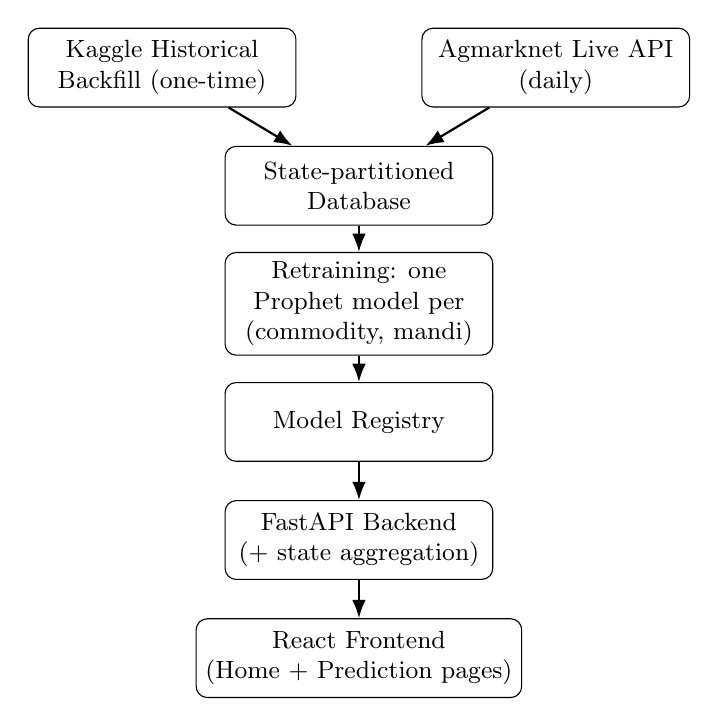
\begin{tikzpicture}[
    box/.style={draw, rounded corners, minimum width=3.4cm, minimum height=1cm, align=center, font=\small},
    arr/.style={-Latex, thick}
]
\node[box] (kaggle) at (0,6) {Kaggle Historical\\Backfill (one-time)};
\node[box] (live) at (5,6) {Agmarknet Live API\\(daily)};
\node[box] (db) at (2.5,4.5) {State-partitioned\\Database};
\node[box] (train) at (2.5,3) {Retraining: one\\Prophet model per\\(commodity, mandi)};
\node[box] (registry) at (2.5,1.5) {Model Registry};
\node[box] (api) at (2.5,0) {FastAPI Backend\\(+ state aggregation)};
\node[box] (frontend) at (2.5,-1.5) {React Frontend\\(Home + Prediction pages)};

\draw[arr] (kaggle) -- (db);
\draw[arr] (live) -- (db);
\draw[arr] (db) -- (train);
\draw[arr] (train) -- (registry);
\draw[arr] (registry) -- (api);
\draw[arr] (api) -- (frontend);
\end{tikzpicture}
\caption{Proposed system architecture: data sources, storage, model
training/registry, API, and frontend.}
\label{fig:architecture}
\end{figure}

An important design decision, discussed further in Section~3.4, is that
\textbf{storage and the user interface are organized by state}, while the
\textbf{forecasting model itself remains at (commodity, mandi)
granularity} -- state-level views are computed as an aggregation over
underlying mandi-level forecasts rather than being separately modelled.

\section{Data Pipeline}
\subsection{Historical Backfill}
Prophet requires several months of history to reliably detect weekly and
yearly seasonality; this cannot be obtained from live daily collection
alone within a single academic year. The system therefore performs a
one-time historical backfill from the Kaggle "Daily Market Prices of
Commodity India (2001--2026)" dataset -- specifically its 2024 and 2025
slices -- before daily live collection begins. This dataset is compiled
by the same original maintainer as the live Agmarknet API dataset used
for daily ingestion, giving one consistent data lineage across historical
and live collection.

\subsection{State and Crop Selection}
The three states and six crops per state (Table~\ref{tab:cropselection})
were finalized by ranking commodities within the 2024+2025 backfill data
by total reported record count per commodity per state (aggregated
across all mandis and days), with mandi count and day count examined
alongside as supporting context. For Tamil Nadu, whose top commodities
were closely clustered in volume, rankings were computed on combined
2024+2025 totals rather than a single year, since single-year rankings
shifted noticeably between the two years; Uttar Pradesh and Maharashtra
produced the same top-6 ranking independently in both years and did not
require this adjustment.

\begin{longtable}{@{}p{2.8cm}p{10.5cm}@{}}
\toprule
\textbf{State} & \textbf{Top 6 crops (ranked)} \\
\midrule
\endhead
Tamil Nadu & Coconut; Bhindi (Ladies Finger); Green Chilli; Bottle gourd;
Snakeguard; Onion (edged out Banana-Green by a narrow margin, ranked on
combined 2024+2025 data) \\
Uttar Pradesh & Potato; Onion; Tomato; Wheat; Brinjal; Green Chilli
(stable ranking independently in both 2024 and 2025) \\
Maharashtra & Wheat; Bengal Gram; Soyabean; Arhar (Tur/Red Gram); Onion;
Jowar (Sorghum) (stable ranking independently in both 2024 and 2025) \\
\bottomrule
\caption{Finalized state and top-6-crop selection, ranked by total
reported record count on the 2024+2025 backfill data.}
\label{tab:cropselection}
\end{longtable}

\subsection{Live Ingestion}
A scheduled job (GitHub Actions cron) fetches the previous day's records
from the Agmarknet API (resource ID
\texttt{9ef84268-d588-465a-a308-a864a43d0070}) and appends them to the
same state-partitioned tables used by the historical backfill, so that
the model's training set grows continuously.

\subsection{Data Cleaning Considerations}
Preliminary analysis of a sample Agmarknet export surfaced two practical
issues that the ingestion pipeline must handle:
\begin{itemize}
    \item \textbf{Field-name encoding.} Exported column names contain an
    XML-encoding artefact (e.g.\ \texttt{Min\_x0020\_Price}) rather than
    the clean \texttt{min\_price} field name returned by the JSON API;
    the pipeline must normalize this during ingestion.
    \item \textbf{Variety/grade duplication.} A single (market, commodity,
    date) combination can have multiple rows if more than one
    variety/grade of that commodity was traded that day (confirmed
    empirically, e.g. multiple \textit{Arecanut} rows at the same market
    on the same day with different modal prices). The pipeline filters to
    a consistent variety/grade per (commodity, mandi) series before
    constructing the Prophet training set.
\end{itemize}

\section{Machine Learning Design}
\subsection{Task Formulation}
The core forecasting task is \textbf{time-series regression}, not
classification: the model predicts a continuous value (the next-period
modal price), using \texttt{modal\_price} as the target variable (the
price at which the largest transacted quantity occurred that day, per
Agmarknet convention) rather than the min/max range. The farmer-facing
Sell/Hold/Stable label is a rule-based decision layer applied on top of
the continuous forecast, not a directly trained classifier -- this
preserves the underlying magnitude/confidence information that a bare
label would discard, and mirrors how real trading/advisory systems are
typically structured.

\subsection{Model Choice}
\textbf{Facebook Prophet} (an additive decomposition model: trend +
weekly seasonality + yearly seasonality) is used as the primary
forecasting model, trained independently per (commodity, mandi) pair. A
naive/moving-average baseline is trained alongside it for comparison,
evaluated using Mean Absolute Error (MAE), to provide an evidence-based
justification for the modelling choice rather than an assumed one.

\subsection{State-Level Aggregation (not a separate model)}
The Prediction page's state-level summary view ("select a state, see its
top 6 crops with percentage change") is computed by aggregating the
outputs of the existing per-mandi models -- e.g.\ averaging the forecast
percentage change across all mandis reporting a given commodity within
the selected state -- rather than training a new, coarser model. This
preserves per-mandi precision for the underlying comparison feature while
still providing a fast, simple state-level overview.

\section{Technology Stack}
Table~\ref{tab:techstack} summarizes the finalized technology choices and
their justification.

\begin{longtable}{@{}p{2.8cm}p{3.8cm}p{6.5cm}@{}}
\toprule
\textbf{Layer} & \textbf{Technology} & \textbf{Justification} \\
\midrule
\endhead
Historical backfill & Kaggle "Daily Market Prices of Commodity India" (2024+2025 parquet) & Same lineage/maintainer as live API dataset; bulk-filterable across states/crops \\
Live data source & data.gov.in Agmarknet API & Free, structured, government-maintained \\
Forecasting model & Facebook Prophet & Handles small per-mandi series well; minimal tuning \\
Baseline model & Naive / moving average (scikit-learn) & Enables an evidence-based accuracy comparison \\
Backend & FastAPI (Python) & Lightweight, async, auto-documented REST API \\
Database & SQLite (dev) / Supabase Postgres (prod) & Free hosting; state-partitioned schema \\
Frontend & React (Vite) & Required for interactive, clickable India map \\
Mapping & react-simple-maps + TopoJSON & Standard approach for clickable choropleth/state maps \\
Charting & recharts & React-native price/forecast visualization \\
Scheduling & GitHub Actions & Free CI/CD-based cron scheduling \\
Deployment & Vercel/Netlify (frontend), Render (backend), Supabase (DB) & All free-tier, standard for student deployment \\
\bottomrule
\caption{Finalized technology stack.}
\label{tab:techstack}
\end{longtable}

\section{Feasibility Discussion}
\subsection{Data Feasibility}
Both the live (Agmarknet API) and historical (Kaggle-compiled Agmarknet)
data sources have been confirmed to be freely accessible without
institutional gatekeeping,
unlike domains such as healthcare (patient-data access restrictions) or
finance (proprietary transaction data), which was a key factor in
selecting this domain over alternatives originally considered.

\subsection{Technical Feasibility}
Each component of the proposed stack (Prophet, FastAPI, React) is
well-documented and widely used in comparable applications, keeping the
implementation risk manageable for a team building most of this tooling
for the first time in a practical setting.

\subsection{Timeline Feasibility}
The project scope (2--3 states, six commodities per state, roughly
15--20 mandis per state) was deliberately bounded to fit a single
academic-year capstone timeline, with a clear path to widening coverage
later without architectural change (Section~3.1).

\subsection{Ethical and Regulatory Considerations}
As the system uses only publicly published government price data and
does not process any personal, medical, or financial data, it does not
raise the consent, privacy, or regulatory concerns that a healthcare- or
finance-domain project would.

\chapter{Results, Analysis \& Discussions}

\section{Status as of \ReviewLabel}
At the time of this review, the project is in the architecture and
scaffolding stage: the system design (Chapter~3), data pipeline strategy,
and technology stack have been finalized, and the project's version-control
repository has been structured accordingly (data pipeline, machine
learning, backend, and frontend modules, each with defined interfaces).
Implementation of the live data pipeline, model training, and the
frontend application is in progress and had not yet produced evaluable
output at the time of this submission.

% TODO (Review 2 onward): replace this chapter's content with actual
% results as they become available -- e.g.:
%   - Sample of cleaned, backfilled historical data (row counts, date
%     coverage per state/commodity)
%   - Prophet vs. baseline MAE comparison table, per commodity/mandi
%   - Screenshots of the working dashboard / prediction page
%   - Any deviations from the Chapter 3 design and why

\section{Preliminary Data Analysis}
A sample single-day national Agmarknet export (9{,}584 records across 25
states, 271 districts, 642 markets, and 188 commodities) was analyzed to
validate assumptions made during architecture design. This confirmed, in
particular: (a) the field-name encoding artefact described in
Section~3.2.3 is present in bulk exports and not only the API preview;
(b) the variety/grade duplication pattern occurs in practice (e.g.\ two
distinct modal prices recorded for \textit{Arecanut} at the same market
on the same day); and (c) commodity reporting coverage varies
meaningfully by state -- for example, an originally assumed commodity
(Soyabean) had zero recorded rows for Maharashtra on the sampled day,
which directly motivated the shift to a data-driven, per-state top-crop
selection methodology (Section~3.1) rather than an assumed fixed crop
list.

\section{Discussion}
This preliminary analysis illustrates the value of validating
architectural assumptions against real data before implementation begins
-- several design decisions in Chapter~3 (state-based data organization,
data-driven crop selection, variety-deduplication logic) were refined
directly as a result of this analysis rather than decided purely from
documentation.

\chapter{Conclusion, Future Scope, Limitations}

\section{Conclusion (Current Stage)}
This report has presented the motivation, problem statement, literature
positioning, and complete proposed architecture for the
\ProjectTitle. The system's design -- a state-organized but
mandi-granular forecasting approach, combining a one-time historical
backfill with a continuously updating live pipeline -- was refined
through preliminary analysis of real Agmarknet data rather than fixed
in advance from assumption alone. The project's codebase has been
scaffolded in line with this design and is under active development.

\section{Work Plan and Timeline}
Table~\ref{tab:timeline} presents the project's phase-wise plan and
current status as of \ReviewLabel. Status will be updated at each
subsequent review period.

\begin{longtable}{@{}p{1.2cm}p{7.5cm}p{3cm}@{}}
\toprule
\textbf{Phase} & \textbf{Deliverable} & \textbf{Status} \\
\midrule
\endhead
1 & Supabase connection verified, normalized DB schema (single \texttt{price\_records} fact table, not state-partitioned), Kaggle parquet historical backfill loaded and validated (1,185,657 records, 3 states, 2024-01-01 to 2025-12-29 -- Section~3.2.2) & Done \\
2 & Data-driven top-6-crops-per-state selection (Table~\ref{tab:cropselection}, Chapter~3) & Done \\
3 & Prophet model + naive baseline per (commodity, mandi), MAE comparison & Not Started \\
4 & Sell/Hold decision logic, validated against historical cases & Not Started \\
5 & Retraining pipeline, model registry, state-aggregation logic & Not Started \\
6 & FastAPI backend: per-mandi and state-summary endpoints & Not Started \\
7 & React frontend: Home page & In Progress \\
8 & React frontend: Prediction page (map + drill-down) & Not Started \\
9 & Automated scheduling and deployment & Not Started \\
10 & Polish, documentation, final report & Not Started \\
\bottomrule
\caption{Project phase-wise work plan and status as of \ReviewLabel.}
\label{tab:timeline}
\end{longtable}

\section{Current Limitations}
As the project is at an early implementation stage, the following
limitations apply as of this review and are expected to be resolved in
subsequent phases:
\begin{itemize}
    \item No trained forecasting model exists yet; forecasting accuracy
    cannot be evaluated at this stage (planned for Phase 3).
    \item The live data pipeline and scheduled retraining job are
    currently stub implementations (intentionally not yet scheduled to
    run automatically, to avoid failures on incomplete code).
    \item The frontend currently covers only the Home page structure;
    the interactive India-map prediction page is planned for Phase 8.
    \item Whether multiple reported varieties of the same commodity
    (e.g.\ Onion, Green Chilli) should be collapsed into a single series
    per (commodity, mandi) or modelled separately per variety is not yet
    decided; this affects total model count and will be resolved before
    Phase 3 training begins.
\end{itemize}

\section{Future Scope}
Beyond the current planned scope, the architecture supports several
natural extensions without structural redesign: additional states and
commodities (Section~3.1), explainability layers (e.g.\ SHAP/LIME) for
the forecasting model to support academic evaluation and farmer trust,
SMS/regional-language delivery of Sell/Hold alerts for farmers without
reliable smartphone/internet access, and integration of weather data as
an additional forecasting feature.


% ---------------------------------------------------------------
% BACK MATTER
% ---------------------------------------------------------------
\appendix
\chapter{Appendices}
\addcontentsline{toc}{chapter}{Appendices}

% TODO: add supplementary material as it becomes available, e.g.:
%   - Full data schema / table definitions
%   - Sample raw API responses
%   - Extended tech-stack configuration details
%   - Team member GitHub/contribution summary

\section*{A.1 Repository}
The project's source code and this report's LaTeX source are maintained
at: \url{https://github.com/live-mandi-advisor/live-mandi-price-advisor}


\nocite{*} % TODO: remove once real in-text \cite{} commands are added;
           % this forces the placeholder references to appear for now.
\bibliographystyle{plainnat}
\bibliography{references}

\end{document}
